%20/03 - Carlos Aguirre
\chapter{Teoría de grafos y métricas}
\section{Introducción a la teoría de grafos}
La teoría de grafos ha sido utilizada recientemente para:
\begin{itemize}
\item Clasificación automática de secuencias de proteínas.
\item Detección de jerarquías de proteínas.
\item Análisis de redes genéticas.
\item Reconstrucción de redes genéticas grandes obtenidas mediante modificación de genes.
\end{itemize}

Un grafo G es un par de conjuntos (V,E) donde $V = \{v_1, v_2, \ldots v_n\}$ es el conjunto de vértices o nodos y $E = \{(v_i, v_j), (v_{i'}, v_{j'}), \ldots \}$ es un conjunto de pares no ordenados de elementos de V y se denomina conjunto de ramas del grafo. 
\marginpar[\footnotesize Pregunta de test: define orden y tamaño, dado un grafo dar el orden y tamaño, etc. ]  \
El número de nodos se denomina \textbf{orden} del grafo, y el número de ramas es el \textbf{tamaño} del grafo. 

\begin{figure}[h]
\centering
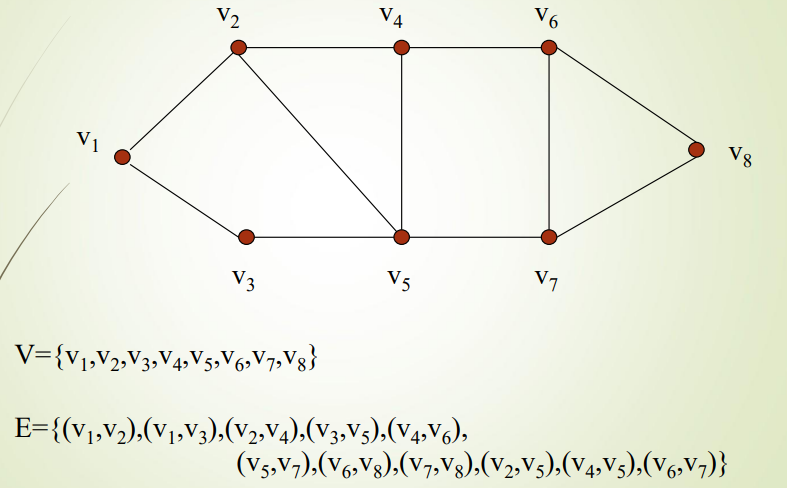
\includegraphics[width = 0.6\textwidth]{figs/grafo.png}
\caption{Ejemplo de grafo de orden 8 y tamaño 11.}
\end{figure}

Para una red de proteínas, cada proteína sería un nodo del grafo, y una rama indicaría interacción entre ambas proteínas. 

Una disposición (layout) es una posible colocación de los nodos y las ramas en un espacio 2D o 3D. Un mismo gráfo puede tener múltiples colocaciones. Ejemplo, consideremos el grafo G=(V,E).

\begin{figure}[h]
\centering
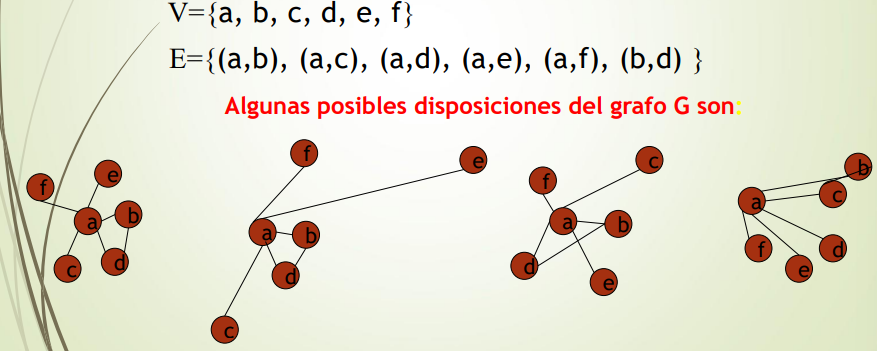
\includegraphics[width = 0.6\textwidth]{figs/layout.png}
\end{figure}

Existen programas de ordenador que nos permiten obtener colocaciones predefinidas (Gephy, Pajek). Cuando no se especifica ninguna colocación, se entiende que los nodos se sitúan aleatoriamente sobre el plano o espacio. Algunos de los tipos más habituales de colocaciones son:
\begin{itemize}
\item Colocaciones regulares
\item Basadas en la física (atracción-repulsión)
\item Basadas en propiedades topológicas (jerarquías, número de vecinos, etc)
\end{itemize}

Un hipergrafo H es un también par de conjuntos (V,E) donde $V=\{v_1, v_2, \ldots v_n\}$ es el conjunto de vértices o nodos y $E=\{(v_{i1}, v_{i2}, \ldots),(v_{i'1},v_{i'2}, \ldots), \ldots\}$ es una familia de
subconjuntos no ordenados de elementos de V. E se denomina conjunto de hiperramas o hiperaristas del hipergrafo. El número de hiperramas $|E|$ se denomina cardinalidad del hipergrafo. El valor $|E|*|V|$ se denomina tamaño o volumen del grafo.
\marginpar[\footnotesize Pregunta examen ]  \
Si tenemos un grafo de n nodos, ¿cuántas parejas podemos tener como máximo? $(n \cdot n-1)/2$ Por tanto, en un grafo con n nodos, ¿cuántas ramas puede tener? Igual, $(n \cdot n-1)/2$

\begin{figure}[h]
\centering
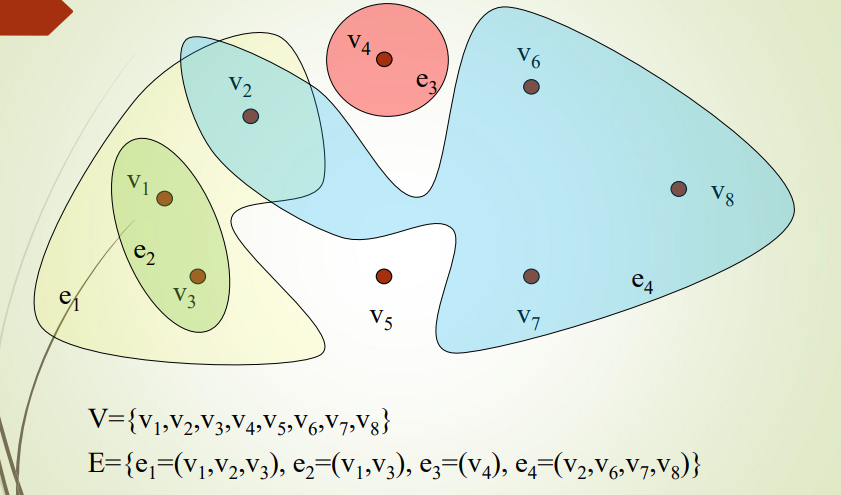
\includegraphics[width = 0.6\textwidth]{figs/hipergrafo.png}
\caption{Ejemplo de hipergrafo de cardinalidad 4 y tamaño 32.}
\end{figure}

Un hipergrafo H se dice que es \textbf{propio} si no es vacío ($V\neq \varnothing$) y no contiene ninguna arista vacía. Un hipergrafo H se dice que tiene \textbf{dominio completo} si todos los nodos están en al menos una arista, en caso contrario se dice que tiene \textbf{dominio parcial}. Si en un hipergrafo todas las hiperramas tienen el mismo número de nodos, entonces se denomina \textbf{hipergrafo k-uniforme}. 

\textit{Ejercicio: Indicar si el hipergrafo del ejemplo anterior es propio, tiene dominio completo y si es k uniforme}. Es propio (el conjunto de vértices tiene 8 elementos y todas las ramas e tienen vértices dentro), es de dominio parcial (v5 no está en ninguna rama) y no es k-uniforme (e1 tiene 3 elementos, e2 tiene 2, e3 tiene 1 y e4 tiene 4).

\section{Bucles y ramas paralelas}
Un bucle es una rama que empieza y termina en el mismo nodo $(v_i, v_i)$. Cuando dos ramas conectan el mismo par de vértices se denominan paralelas. Un grafo con bucles se denomina pseudografo. Un grafo con ramas paralelas pero sin bucles se denomina multigrafos. Un grafo sin bucles ni ramas paralelas se denomina grafo simple.

\begin{figure}[h]
\centering
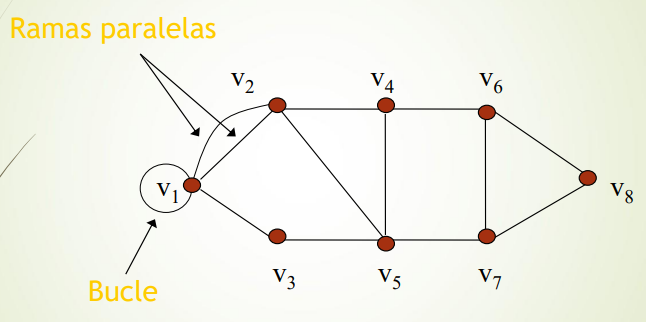
\includegraphics[width = 0.6\textwidth]{figs/bucle-rama-paralela.png}
\end{figure}

%25/03 - Carlos Aguirre
\section{Grafos dirigidos y ponderados}
Se puede considerar que los enlaces entre nodos son dirigidos $(v_i, v_j) = (v_j, v_i)$. Los grafos dirigidos se denominan también \textbf{digrafos}.

\begin{figure}[h]
\centering
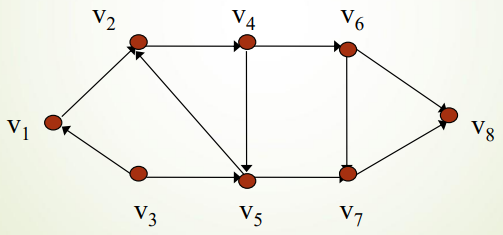
\includegraphics[width = 0.6\textwidth]{figs/grafo-dirigido.png}
\end{figure}

En los grafos ponderados, a cada rama del grafo se le puede asociar un número. El número asociado a cada rama puede indicar entre otras cosas una distancia, una capacidad, un valor temporal, etc.

\begin{figure}[h]
\centering
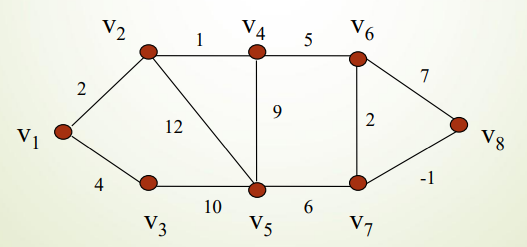
\includegraphics[width = 0.6\textwidth]{figs/grafo-ponderado.png}
\end{figure}

\newpage

Los grafos dirigidos y ponderados poseen ramas dirigidas a las que se asocia un número.

\begin{figure}[h]
\centering
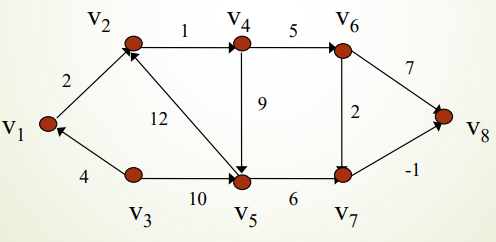
\includegraphics[width = 0.6\textwidth]{figs/grafo-dirigido-ponderado.png}
\end{figure}

\section{Grado de un nodo}
Dos nodos de un grafo son \textbf{vecinos o adyacentes} si existe una rama que los conecta. El \textbf{grado} de un nodo es el número vecinos que tiene dicho nodo. En los grafos dirigidos se calcula el \textbf{grado de entrada} y el \textbf{grado de salida}. En los grafos ponderados, el grado se puede promediar por el número asociado a las ramas. Un grafo se dice que es \textbf{regular} si todos los nodos tienen el mismo grado.

\begin{figure}[h]
\centering
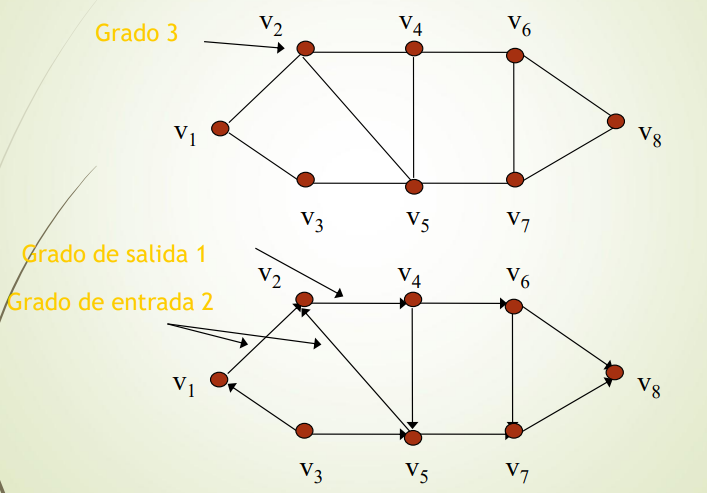
\includegraphics[width = 0.6\textwidth]{figs/grafo-grados.png}
\end{figure}

\section{Subgrafos}
Un grafo G’=(V’,E’) es un subgrafo de un grafo G=(V,E) si V’ es un subconjunto de V y E’ es un subconjunto de E. En otras palabras, un subgrafo es un trozo de un grafo más grande. 

\begin{figure}[h]
\centering
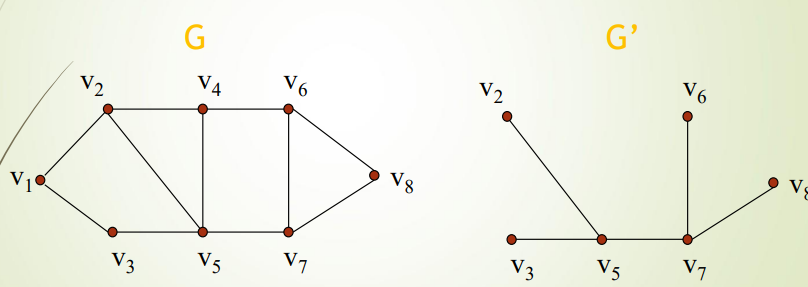
\includegraphics[width = 0.6\textwidth]{figs/subgrafo.png}
\end{figure}

Un subgrafo G’=(V’,E’) de un grafo G=(V,E) se dice que es \textbf{abarcador} si V=V’, es decir, si están todos los nodos, pero faltan algunas ramas.

Un grafo es un subgrafo de sí mismo. Además, un grafo vacío es un subgrafo de cualquier grafo.

\section{Paseos, caminos, circuitos y ciclos}
Un \textbf{paseo} de un nodo u a un nodo v es una secuencia de vértices $\{v_0, v_1, \ldots, v_k\}$ con $v_1 = u v_k = v$ y $(v_{i-1}, v_i)$ rama del grafo. El número de ramas del paseo es su \textbf{longitud}. Un paseo en el cual no se repiten ramas se denomina \textbf{rastro}. Un paseo en el cual todos los vértices $\{v_0, v_1, \ldots, v_k\}$ son distintos se denomina \textbf{camino}. 
Un camino siempre debe ser un rastro y un paseo. Si algo no es rastro, no puede ser camino, y si no es paseo, no puede ser ni rastro ni camino. Cada uno es cada vez más restrictivo.

Entre dos nodos, puede haber varios caminos posibles. Un \textbf{camino mínimo} entre dos nodos es aquel de menor longitud de entre todos los posibles caminos entre ambos nodos. La \textbf{distancia} entre dos nodos del grafo se define como la longitud de cualquier camino mínimo que los una.

\begin{figure}[h]
\centering
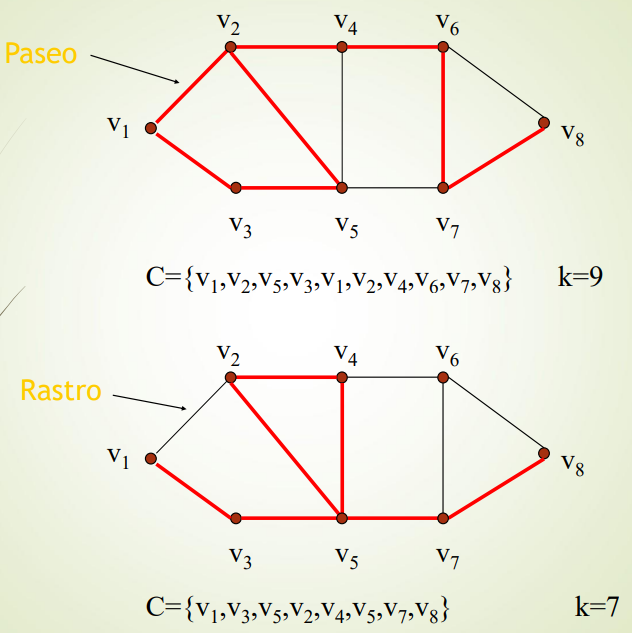
\includegraphics[width = 0.5\textwidth]{figs/paseo-rastro.png}
\end{figure}

\begin{figure}[h]
\centering
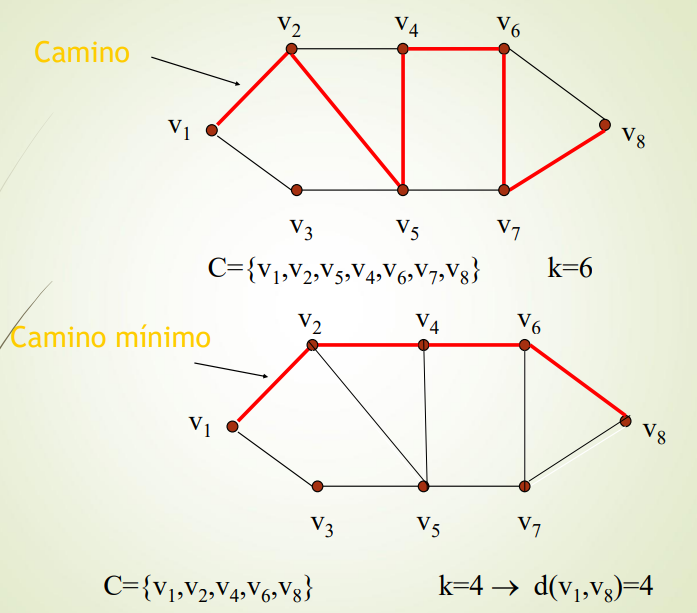
\includegraphics[width = 0.5\textwidth]{figs/camino-minimo.png}
\end{figure}

Un \textbf{paseo cerrado} es un paseo $\{v_0, v_1, \ldots, v_k\}$ tal que $v_0 = v_k$. Un paseo cerrado en el que no se repiten ramas es un \textbf{circuito}. Un \textbf{ciclo} es un circuito en el que no se repiten vértices. Los ciclos son importantes, porque las redes biológicas tienen ciclos (que suelen ser largos), pero en las redes aleatorias no aparecen ciclos, o éstos son muy pequeños.

\begin{figure}[h]
\centering
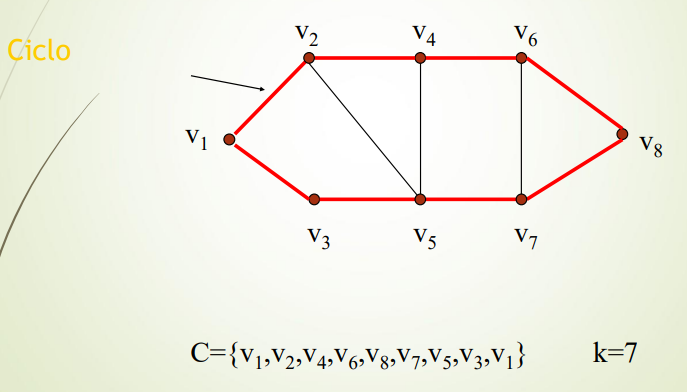
\includegraphics[width = 0.5\textwidth]{figs/ciclo.png}
\end{figure}

El nodo con menor distancia entre los demás es muy importante, denominándose como \textbf{centro del grafo}.

Para un grafo con excesivos nodos, los caminos mínimos y las distancias se calculan con un algoritmo. Si el grafo es no ponderado, se utiliza el algoritmo búsqueda en anchura, mientras que si es ponderado, utiliza Dijkstra.

\section{Medidas de centralidad, betweeness y closeness}
\marginpar[\footnotesize Pregunta examen: Betweeness/Closeness/Farness se define como... ]  \
Dado un nodo $v_i$ se define su \textbf{betweeness} $C_B (v_i)$ como la fracción de caminos mínimos que hay entre el resto de nodos del grafo y que pasan por el nodo $v_i$. Es decir, se hacen parejas de todos los nodos del grafo excluyendo el nodo de interés, y se calculan los caminos mínimos. Algunos pasarán por el nodo de interés, que son los que nos quedamos. Con eso se evalúa el cociente (los que pasan por ese nodo entre todos), que será el betweeness (un valor entre 0 y 1).
La centralidad de un nodo es muy costosa de calcular, usualmente se emplean algoritmos aproximados. 

Dado un nodo $v_i$ se define su \textbf{lejanía o farness} $C_F (v_i)$ como la suma de las distancias de $v_i$ al resto de nodos del grafo. 

Dado un nodo $v_i$ se define su \textbf{cercanía o closeness} $C_C (v_i)$ como la inversa de su lejanía $C_C (v_i) = 1/C_F (v_i)$.

\begin{figure}[h]
\centering
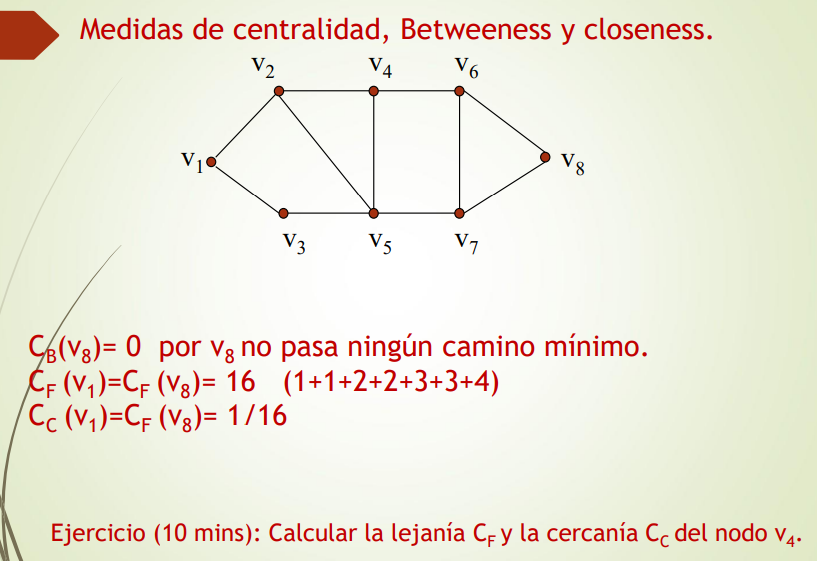
\includegraphics[width = 0.5\textwidth]{figs/medidas-centralidad.png}
\caption{Respuesta al ejercicio: Cogiendo v4, la lejanía será 2+1+2+1+1+2+2 = 11, y la cercanía 1/11.}
\end{figure}

La cercanía y lejanía tiene un problema: su valor numérico depende del orden del grafo. Por tanto, sirve para comparar dentro del mismo grafo, pero no entre grafos. 
\marginpar[\footnotesize Pregunta examen: Calcular camino característico ] \
Para eso, habría que normalizar dividiendo por el número total de nodos. A esto se le conoce como \textbf{camino característico}.

\section{Conexidad}
Un grafo es \textbf{conexo} si para cada par de nodos del grafo existe al menos un camino que los une. En otras palabras, que no esté separado en distintos trozos. 

\begin{figure}[h]
\centering
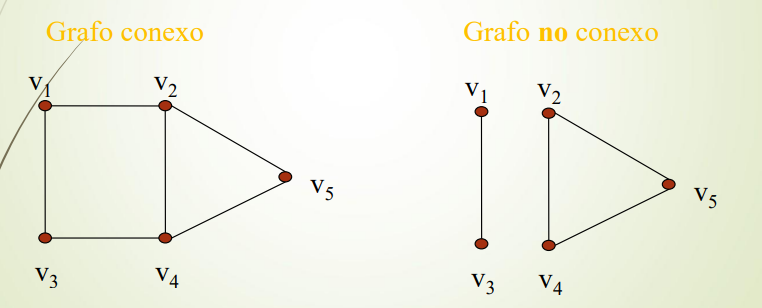
\includegraphics[width = 0.6\textwidth]{figs/conexidad.png}
\end{figure}

Hay un algoritmo muy rápido y eficiente que calcula si un grafo es conexo o no. 

Una \textbf{componente conexa} de un grafo es cada uno de los subgrafos
maximales conexos. Esto quiere decir que el subgrafo no puede ser más grande, que no se le puede añadir más nodos.

\begin{figure}[h]
\centering
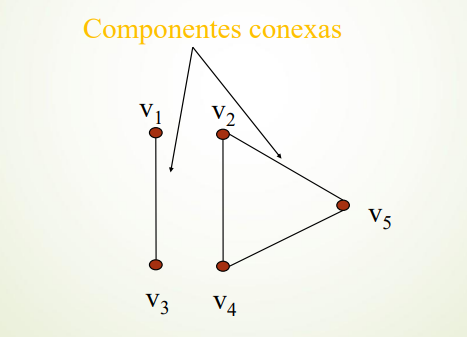
\includegraphics[width = 0.5\textwidth]{figs/componentes-conexas.png}
\end{figure}

Un \textbf{punto de articulación} es un nodo que desconecta un grafo conexo. Un \textbf{corte} es un conjunto de ramas que desconecta un grafo conexo. Si un corte esta compuesto por una única rama, se denomina \textbf{puente}. Un \textbf{corte mínimo} de un grafo es el mínimo número de ramas que al ser eliminadas desconectan el grafo.

El algoritmo CLICK (CLuster Identification via Connectivity Kernels) calcula una aproximación al corte mínimo. Esto lo hacían cogiendo los dos nodos más lejanos. Los puentes suelen ser muy malos para la conexidad de los grafos. 

\begin{figure}[h]
\centering
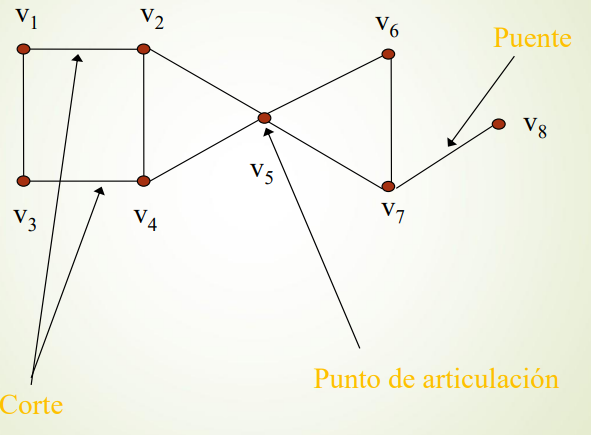
\includegraphics[width = 0.5\textwidth]{figs/conexidad2.png}
\end{figure}

La máxima distancia entre cualquier par de nodos se denomina como diámetro.

El corte mínimo entre dos nodos es siempre mayor que el corte mínimo de todo el grafo.  

\section{Bosques y árboles}
Un grafo sin ciclos (acíclico) se denomina bosque. Un árbol es un grafo acíclico conexo. Cada componente conexa de un bosque es un árbol.

\begin{figure}[h]
\centering
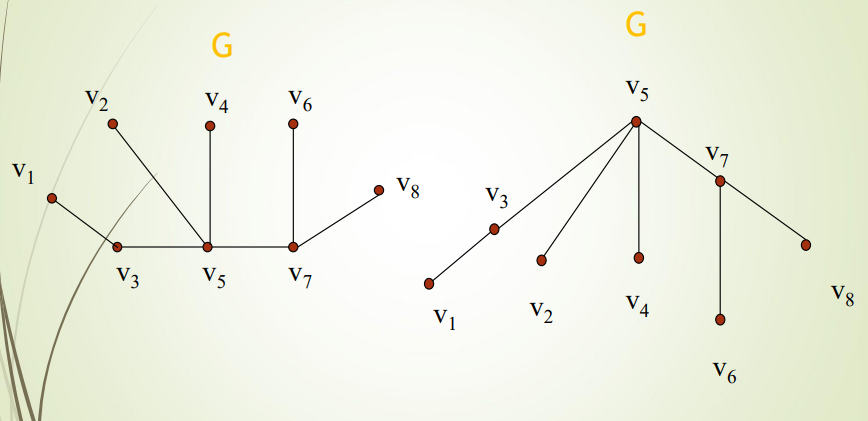
\includegraphics[width = 0.6\textwidth]{figs/arbol-bosque.png}
\end{figure}

Un subgrafo abarcador acíclico de un grafo G se denomina un \textbf{bosque abarcador}. Un subgrafo abarcador conexo acíclico de un grafo G se denomina un \textbf{árbol abarcador}.

\begin{figure}[h]
\centering
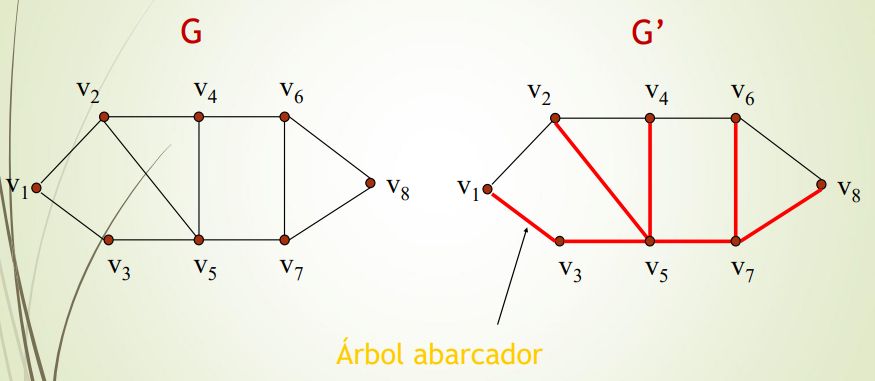
\includegraphics[width = 0.6\textwidth]{figs/arbol-abarcador.png}
\end{figure}

%27/03 - Carlos Aguirre
\section{Grafos bipartitos}
Un grafo se dice que es bipartito si:
\begin{itemize}
\item El conjunto de vértices V se puede romper en dos subconjuntos disjuntos V1 y V2.
\item El vértice inicial de cada rama de E pertenece a V1 y el vértice final a V2
\end{itemize}

Ejercicio: el grafo anterior (el del árbol abarcador), ¿es bipartito? No, porque no es posible realizar la partición. Si V1 pertenece al conjunto 1, V2 y V3 deben estar en el conjunto 2, por lo que V4 y V5 tienen que estar en V1, pero esto no es posible porque están conectados entre sí. La condición necesaria para que un grafo sea bipartito es que no tenga triángulos. Pero esto no es suficiente; se puede construir un grafo sin triángulos, pero que tampoco sea bipartito. Si cogemos solo el cuadrado V4-V7, sí se podría generar un grafo bipartito: V4 y V7 en un conjunto y V5 y V6 en otro. 

\section{Representación de grafos}
Hay dos formas estándar de representar un grafo en un ordenador:
\begin{itemize}
\item \textbf{Matriz de adyacencia}: consume mucha memoria, pero es fácil de añadir o eliminar ramas. Es fácil saber si existe una rama, pero es lento enumerar los vecinos de un nodo. Se pueden calcular los autovalores y autovectores.
\item \textbf{Lista de adyacencia}: tiene un consumo limitado de memoria, pero es costoso añadir o eliminar ramas. También es costoso saber si existe una rama, pero rápido enumerar los vecinos de un nodo.
\end{itemize}

\section{Métricas sobre grafos}
Los grafos se clasifican en función de unas determinadas métricas topológicas. Las métricas más empleadas son:
\begin{itemize}
\item Tamaño |E| y orden |V|
\item Dispersión: $\frac{2 |E|}{|V| (|V| - 1)}$ para un grafo no dirigido y $\frac{|E|}{|V| (|V| - 1)}$ para un grafo dirigido. Si el coeficiente es pequeño (0), el grafo es disperso, si es cercano a 1, es denso. En redes biológicas, los grafos suelen ser dispersos.
\item Distribución del grado de los nodos: división del grado de todos los nodos entre el número de nodos. El resultado es una distribución de probabilidad. En un grafo aleatorio, la distribución es de Poisson (como la gaussiana, pero sin valores negativos). En las redes biológicas, la distribución no será de Poisson, por lo que este será el primer test que se haga a los datos. 
\item Grado medio (<k>): media del grado de todos los nodos.
\item Coeficiente de agrupamiento (C)
\marginpar[\footnotesize Pregunta examen: Calcular C o L de un grafo ] \
\item Camino característico (L)
\end{itemize}

%01/04 - Carlos
\subsection{Coeficiente de agrupamiento C}
El coeficiente de agrupamiento (C) es un valor métrico \textbf{local} que mide el nivel de agrupamiento de los nodos. Es decir, mira un nodo y sus vecinos y mira el índice de clusterización. En redes biológicas, el índice de clusterización es alto. Para cada nodo v del grafo se obtiene su vecindario, es decir, el conjunto de nodos que son vecinos de v, el tamaño del vecindario coincide con el grado de v (kv). Se calcula el coeficiente
$$Cv = \frac{Nv}{kv(kv-1)/2} = \frac{\text{número real de ramas entre vecinos sin incluir el nodo v}}{\text{número máximo de ramas entre vecinos}}$$
donde Nv es el numero de ramas que hay entre los vecinos de v. El valor anterior se promedia entre todos los nodos del grafo. 

\begin{figure}[h]
\centering
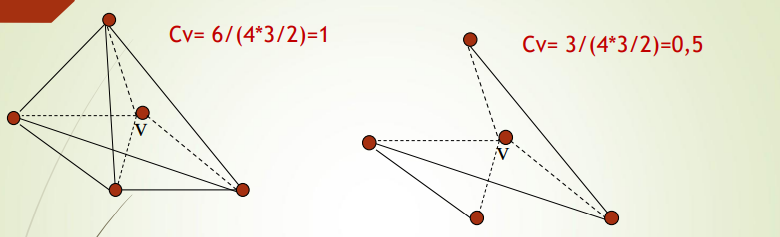
\includegraphics[width = 0.8\textwidth]{figs/coeficiente-agrupamiento.png}
\caption{Figura de la izquierda: todos los vecinos del nodo v son vecinos entre sí. Figura de la derecha: la mitad de mis amigos son amigos entre sí (0,5).}
\end{figure}

Para un grafo, se calcula el coeficiente de agrupación es el valor de cada nodo dividido por el número de nodos - es decir, el promedio. Para simetría, se calcula el valor de una fracción de los nodos y se divide por esa fracción.

Ejercicio: calcular el coeficiente de agrupamiento C del siguiente grafo. Se sugiere utilizar simetrías para reducir el trabajo. Esto será igual en el examen. 

\begin{figure}[h]
\centering
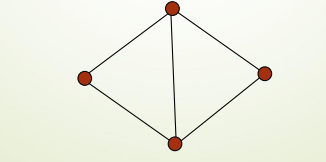
\includegraphics[width = 0.3\textwidth]{figs/ejercicio-calculo-c.png}
\caption{Se deben calcular dos índices de clusterización: nodo superior (igual al nodo inferior) y nodo izquierdo (igual al nodo derecho). Empezando por el nodo superior, la fórmula quedaría como $2/(3*2/2) = 2/3 = 0,66$. Para el nodo izquierdo, quedaría $3/(3*2/2) = 1$. Ahora hay que sumar esos dos valores y dividir entre el número de nodos calculados: $(1 + 0,66)/ 2 = 1,66/2 = 0,83$.}
\end{figure}

\subsection{Camino característico L}
El camino característico (L) es un valor métrico \textbf{global} que mide el nivel grado de separación de los nodos. Para cada nodo v se calcula la distancia promedio a todos los demás nodos del grafo:
$$Lv = \sum^{|v|}_{k=1} d(v, v_k) / (|v| - 1)$$

Se calcula el promedio del valor anterior entre todos los nodos del grafo. Es como un farness normalizado al número de nodos del grafo.
$$L = \sum^{|v|}_{v=1} L_v / (|v| - 1)$$

En las redes biológicas, el camino característico suele ser cortito. 

Ejercicio: Calcular el camino característico L del grafo de la figura anterior. Se puede (y debe) volver a utilizar simetrías. 
$$L_{v1} = L_{v3} = 1/3 + 1/3 + 1/3 = 1$$
$$L_{v2} = L_{v4} = 1/3 + 1/3 + 2/3 = 4/3 = 1,33$$
$$L = 1/4 + 1,33/4 + 1/4 + 1,33/4 = 7/6 = 1,165$$

\section{Topologías}
\subsection{Grafos aleatorios}
Fueron estudiados principalmente por Erdos y Renyi en los años 50. Cada rama del grafo existe con una determinada probabilidad p. Erdos y Renyi estudiaron los valores de las métricas topológicas para diferentes valores de $p$. Para la grafos dispersos (p pequeña) se puede comprobar que tanto C (aproximadamente 0) como L (aproximadamemte Ln(|V|) son pequeños.

\subsection{Grafos regulares}
Son los mejor conocidos de forma analítica. Existen expresiones cerradas para todas las métricas. Para la grafos dispersos se puede comprobar que tanto C (aproximadamente 0.75) como L (aproximadamente |V|/<k>) son grandes. 

\subsection{Mundo pequeño}
Son grafos que presentan altos valores de C (aprox .8) y bajos valores de L (aprox ln(|V|). Se obtienen introduciendo un pequeño número de “atajos” en un grafo regular. Representan bien un gran número de redes tales como redes sociales.

Las redes biológicas son todas de mundo pequeño. 

Un grafo de mundo pequeño es aquel cuyo índice de clusterización es el mismo de un grafo regular con el mismo número de nodos y ramas, y cuyo camino característico es el mismo de un grafo aleatorio con el mismo número de nodos y ramas. 

\subsection{Grafos libres de escala}
Son grafos que presentan bajos valores de C (aprox 0) y bajos valores de L (aprox ln(|V|). Se obtienen mediante crecimiento de la red y enlace preferencial. Cuando la distribución de los nodos se dibuja en escala log-log aparece una línea recta. Representan bien un gran número de redes tales como internet o redes de reacciones químicas.

Para diferenciar estas redes de un grafo aleatorio en la escala log-log, ya que los grafos libre de escala son una recta mientras que los aleatorios siguen una distribución de Poisson.

\begin{figure}[h]
\centering
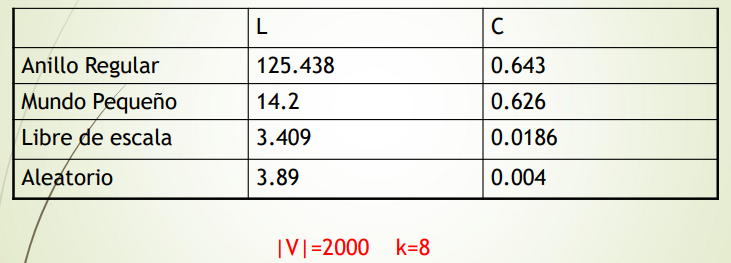
\includegraphics[width = 0.8\textwidth]{figs/metricas-estandar.png}
\end{figure}

Un grafo con 2000 vecinos en el que cada nodo tiene 8 vecinos, ¿cuántas ramas tiene el grafo? 8000. De cada nodo entran y salen 8 ramas. $8 \cdot 2000/2$ porque cada rama se cuenta dos veces, una en cada vecino.

\section{Algoritmos sobre grafos}
El algoritmo de \textbf{búsqueda en anchura} permite calcular un camino mínimo entre dos nodos de un grafo. Dijkstra es una versión del algoritmo anterior para grafos ponderados. Ambos algoritmos funcionan tanto en grafos dirigidos como no dirigidos. Los algoritmos nos permiten calcular las métricas sobre el grafo.

Si los grafos tienen bucles y ramas paralelas, el algoritmo no funciona. 

%08/04 - Carlos
En el algoritmo de búsqueda en anchura, se marcan los nodos vecinos. Símil con los corredores de la antigua Grecia: las noticias se transmitían por los corredores. Había en una ciudad tantos corredores como ciudades vecinas que tenía una ciudad. Si Atenas está siendo invadida por los turcos, no se necesita ningún corredor que vaya a Atenas. Los corredores de Atenas van a los vecinos, marcándolos como visitados y añadiéndolos en la cola. Una vez terminado, se repite con los vecinos de los vecinos de Atenas, así hasta haber completado el grafo.

El algoritmo de Búsqueda en profundidad permite calcular puntos de articulación de un grafo.
El algoritmo de Ford-Fulkerson permite calcular cortes mínimos.

\section{Cálculos sobre grafos: NetworkX}
Existen multitud de herramientas para facilitar el cálculo de las diferentes métricas sobre grafos.
Algunas herramientas también permiten la visualización de grafos de orden y/o tamaño reducido.
Las herramientas pueden ser de tipo interactivo o librerías que se pueden emplear sobre lenguajes de programación.

NetworkX es un paquete Python orientado al análisis de grafos. Permite la creación de digrafos, multigrafos y pseudografos. Además incorpora el cálculo de un elevado número de métricas y algoritmos sobre el grafo. Sin embargo, da un soporte muy reducido a la visualización de grafos mediante el paquete Matplotlib.

\textit{La parte práctica se encuentra en la carpeta ejercicios en el fichero nx.ipynb.}

\subsection{Creación de grafos}
NetworkX permite la creación de grafos mediante tres métodos:
\begin{itemize}
\item \textbf{Creación de un grafo vacío al que posteriormente se añaden nodos y ramas}: se pueden usar varias funciones en networkx: \texttt{Graph}, \texttt{DiGraph}, \texttt{MultiGraph}, \texttt{MultiDiGraph}. Para añadir nodos a un grafo existente podemos usar las siguientes funciones del objeto graph: \texttt{add\_node(n)} donde n puede ser cualquier objejo hashable (int, str, estructura, grafo) y \texttt{add\_nodes\_from(container)} donde container puede ser cualquier objeto contenedor (una lista, conjunto, fichero, nodos de otro grafo).

Pregunta: Si H y G son dos grafos creados previamente, ¿Cuál es la diferencia entre H.AddNode(G) y H.AddNodesFrom(G)? H.AddNode(G) agregaría G como un solo nodo al grafo H, considerándose como una entidad individual. Por el contrario, H.AddNodesFrom agrega todos los nodos de G al grafo H como nodos individuales, es decir, cada nodo de G se copia a H.

Para añadir ramas a un grafo existente se puede utilizar \texttt{add\_edge(n1, n2} y si uno de los dos vértices no existe, se añade al grafo, o \texttt{add\_edges\_from(container} donde container puede ser una lista o colección de ramas. Las propiedades nodes y edges del grafo nos devuelven respectivamente la lista de vértices y ramas del grafo.

A cada objeto del grafo (el propio grafo, los vértices o las ramas) se le puede asignar uno o
varios \textbf{atributos}. Un atributo es un objeto de la forma clave=valor, la clave debe ser un objeto hashable. Los atributos se pueden asignar durante la creación del objeto o una vez creado.

\item \textbf{Creación de un grafo con una topología predefinida}: NetworkX premite la creación de grafos con topologías predefinidas. Los grafos predefinidos están clasificados por categorías, entre otras grafos generales, mallas, grafos aleatorios, árboles, redes sociales, geométricos, comunidades, grafos pequeños, etc.

Para grafos generales, se puede crear un grafo completo (cliqué) con n vértices con \texttt{complete\_graph(n)}. Para crear una cadena con n vértices se utiliza \texttt{path\_graph(n)}. \texttt{cycle\_graph(n)} es lo mismo que el anterior, pero en el cual el primer y último nodo es el mismo. En ambos casos habrá n-1 ramas. \texttt{graph\_atlas(n)} crea un grafo número n del libro An Atlas of Graphs (en el cual el grafo 1 está vacío, el grafo 2 tiene un nodo, el grafo 3 tiene dos nodos pero sin conectar, el grafo 4 tiene dos nodos conectados, etc). 

Las mallas se pueden crear con las funciones \texttt{grid\_2d\_graph(m, n, periodic=false)}, \texttt{grid\_graph} y \texttt{hypercube\_graph(n)}.

Para grafos aleatorios, \texttt{gnp\_random\_graph(n, p)} se crea un grafo con n nodos donde cada una de las posibles ramas del grafo existe con probabilidad p y no estará con probabilidad 1-p.  De media, habrá (p * n * n-1) / 2  ramas. 
\marginpar[\footnotesize Pregunta examen: gnp random graph vs gnm random graph, ramas en gnp random graph] \
La función \texttt{gnm\_random\_graph(n, m)} crea un grafo aleatorio con n nodos y m ramas. La topología generada es la misma que en la función gnp, pero es difícil de demostrar.  \texttt{watts\_strogatz\_graph(n, k, p)} crea un grafo de mundo pequeño con n nodos, cada uno conectado a k vecinos, y p la probabilidad de reconexión de cada nodo. Por último, \texttt{barabase\_albert\_graph(n, m)} crea un grafo libre de escala con n nodos y m ramas.

Se puede crear un árbol aleatorio de n nodos con \texttt{random\_tree(n)}. También está la función \texttt{prefix\_tree(path)} para crear un árbol prefijo generado a partir del iterable de listas path.

\item \textbf{Carga de un grafo desde un fichero externo}
\end{itemize}

\subsection{Importación y exportación de grafos}
NetworkX permite importar grafos y exportar grafos a un fichero con diferentes formatos, los más usuales son adjacency list, multiline adjacency list, edge list, GEFX y otros formatos como JSON, YAML, Pajek, etc.

En la lista de adyacencia, cada línea del fichero representa la lista de adyacencia de un nodo, el primer elemento es el identificador del nodo y a continuación los identificadores de sus vecinos.
La lectura y escritura del fichero se realiza mediante las siguientes funciones:
\begin{itemize}
\item read\_adjlist(path[, comments, delimiter, …]): Lee el grafo indicado por el fichero path.
\item write\_adjlist(G, path[, comments, …]): Guarda el grafo G en el fichero indicado por path.
\item parse\_adjlist(lines[, comments, delimiter, …]): Interpreta las líneas de un grafo representado mediante lista de adyacencia.
\item generate\_adjlist(G[, delimiter]): Genera una línea del grafo G en formato de lista de adyacencia.
\end{itemize}

La lista de adyacencia multillinea incluye cada vecino en una línea separada, siendo útil cuando los índices son cadenas. La lectura y escritura del fichero se realiza mediante las siguientes funciones:
\begin{itemize}
\item read\_multiline\_adjlist(path[, comments, delimiter, …]): Lee el grafo indicado por el fichero path.
\item write\_multiline\_adjlist(G, path[, comments, …]): Guarda el grafo G en el fichero indicado por path.
\item parse\_multiline\_adjlist(lines[, comments, delimiter, …]): Interpreta las líneas de un grafo representado mediante lista de adyacencia multilinea.
\item generate\_multiline\_adjlist(G[, delimiter]): Genera una línea del grafo G en formato de lista de adyacencia multilinea.
\end{itemize}

La lista de ramas contiene una línea para cada rama más sus posibles atributos. Una posible línea podría ser \texttt{a b \{'weight':7, 'color':'green'\}}.  La lectura y escritura del fichero se realiza mediante las siguientes funciones:
\begin{itemize}
\item read\_edgelist(path[, comments, delimiter, …]): Lee el grafo indicado por el fichero path.
\item write\_edgelist(G, path[, comments, …]): Guarda el grafo G en el fichero indicado por path.
\item read\_weighted\_edgelist(path[, comments, delimiter, …]): Lee el grafo ponderado indicado por el fichero path.
\item write\_weighted\_edgelist(G, path[, comments, …]): Guarda el grafo ponderado G en el fichero indicado por path.
\item parse\_edgelist(lines[, comments, delimiter, …]): Interpreta las líneas de un grafo representado mediante lista de ramas.
\item generate\_edgelist(G[, delimiter]): Genera una línea del grafo G en formato de lista de ramas.
\end{itemize}

\subsection{Información sobre el grafo}
NetworkX incorpora una serie de funciones que permiten obtener información sobre el propio grafo, los nodos o las ramas. Las principales funciones de \textbf{información sobre el grafo} son:
\begin{itemize}
\item degree(G[, nbunch, weight]): Devuelve el grado de un nodo o de un grupo de nodos.
\item degree\_histogram(G): Devuelve la distribución de grado del grafo.
\item density(G): Devuelve la densidad del grafo.
\item info(G[, n]): Devuelve un conjunto de información sobre el grafo G o el nodo n.
\item is\_directed(G): Devuelve True si el grafo es dirigido.
\end{itemize}

Las principales funciones de \textbf{información sobre los vértices} son:
\begin{itemize}
\item nodes(G) Devuelve un iterator sobre los nodos del grafo.
\item number\_of\_nodes(G) Devuelve el orden del grafo.
\item all\_neighbors(graph, node) Devuelve todos los vecinos de un vértice.
\item non\_neighbors(graph, node) Devuelve los no-vecinos de un vértice.
\item common\_neighbors(G, u, v) Devuelve los vértices comunes a dos vértices.
\end{itemize}

Las principales funciones de \textbf{información sobre las ramas} son:
\begin{itemize}
\item edges(G[, nbunch]) Devuelve las ramas del grafo entre los vertices indicados en nbunch (todas si no se indica nbunch).
\item number\_of\_edges(G) Tamaño del grafo.
\item non\_edges(graph) Devuelve las ramas que no están en el grafo.
\end{itemize}

Las principales funciones de \textbf{gestión de atributos} son:
\begin{itemize}
\item set\_node\_attributes(G, values[, name]) Establece los atributos de un vértice desde un valor o un diccionario de valores.
\item get\_node\_attributes(G, name) Obtiene los atributos de un vértice
\item set\_edge\_attributes(G, values[, name]) Establece los atributos de una rama desde un valor o un diccionario de valores.
\item get\_edge\_attributes(G, name) Obtiene los atributos de una rama
\end{itemize}

\subsection{Visualización}
NetworkX permite una visualización muy simple (pero a veces suficiente) del grafo. Cuando se desea una visualización más avanzada se suelen realizar los cálculos necesarios con NetworkX y luego el grafo se exporta a otras herramientas como Gephy o Cytoscape. La visualización siempre debe realizarse de grafos o subgrafos pequeños, los algoritmos de visualización son lentos y poco eficientes.

Las principales primitivas de visualización son:
\begin{itemize}
\item draw(G[, pos, ax]): Dibuja el grafo G con Matplotlib, no dibuja colores, ni etiquetas.
\item draw\_networkx(G[, pos, arrows, with\_labels]): Dibuja el grafo G con Matplotlib, permite añadir etiquetas a los objetos
\item draw\_networkx\_nodes(G, pos[, nodelist, …]): Dibuja los nodos del grafo G en las posiciones indicadas por pos.
\item draw\_networkx\_edges(G, pos[, edgelist, …]): Dibuja las ramas del grafo G en las posiciones indicadas por pos.
\item draw\_networkx\_labels(G, pos[, labels, …]): Dibuja las etiquetas de los nodos del grafo G en las posiciones indicadas por pos.
\item draw\_networkx\_edge\_labels(G, pos[, …]): Dibuja las etiquetas de las ramas del grafo G en las posiciones indicadas por pos.
\end{itemize}

NetworkX permite algunos \textbf{layouts} muy simples:
\begin{itemize}
\item draw\_circular(G, **kwargs): Layout circular.
\item draw\_kamada\_kawai(G, **kwargs): Layout dirigido por fuerzas Kamada-Kawai.
\item draw\_random(G, **kwargs): Layout aleatorio.
\item draw\_spectral(G, **kwargs): Layout espectral.
\item draw\_spring(G, **kwargs): Layout de muelle.
\item draw\_shell(G, **kwargs): Layout tipo concha.
\end{itemize}

También es posible recuperar la lista de posiciones de los nodos sin pintarlos, las rutinas devuelven un diccionario con las posiciones de cada nodo.
\begin{itemize}
\item circular\_layout(G, [, scale, center, dim]): Layout circular.
\item kamada\_kawai\_layout (G, [, scale, center, dim]): Layout dirigido por fuerzas Kamada-Kawai.
\item random\_layout (G, [, scale, center, dim]): Layout aleatorio.
\item spectral\_layout (G, [, scale, center, dim]): Layout espectral.
\item spring\_layout (G, [, scale, center, dim]): Layout de muelle.
\item shell\_layout (G, [, scale, center, dim]): Layout tipo concha.
\item rescale\_layout(pos[, scale]) Devuelve el array de numpy pos reescalado a (-scale, scale) en todos los ejes.
\end{itemize}

\subsection{Algoritmos}
NetworkX incluye una cantidad enorme de algoritmos aplicables a grafos (actualmente
unos 250 algoritmos). Los algoritmos se clasifican por categorías en función del problema que resuelven. NetworkX tiene algoritmos en 50 categorías diferentes. Cada una de estas 50 categorías está a su vez dividida en subcategorías. Las categorías más utilizadas en bioinformática son algoritmos para centralidad, cliqués, clustering, conectividad, k-cores, operadores, caminos mínimos, árboles y algoritmos aproximados (problemas Np completo como el cálculo del betweeness).

\subsubsection{Centralidad}
La centralidad de grado es la fracción de los nodos con los que está conectado cada nodo. Están las funciones degree\_centrality, in\_degree\_centrality y out\_degree\_centrality. 

La centralidad de carga es similar al betweenness, pero usa un algoritmo diferente propuesto por Newman. Se puede obtener con load\_centrality para nodos y edge\_load\_centrality para las ramas.

El closeness tiene la función closeness\_centrality. El betweenness se puede calcular con varias funciones: betweenness\_centrality, edge\_betweenness\_centrality, betweenness\_centrality\_subset y edge\_betweenness\_centrality\_subset.

%06/05 - Carlos Aguirre
\subsubsection{Cliqués}
Un cliqué es un subgrafo completo, es decir, un subgrafo en el que todos los nodos están unidos con todos. enumerate\_all\_cliques(G) devuelve todos los cliques de un grafo no dirigido. find\_cliques(G) devuelve los cliqués maximales para cada nodo del grafo. make\_max\_clique\_graph devuelve el cliqué maximal del grafo, y graph\_clique\_number el orden del cliqué maximal del grafo.

\subsubsection{Clustering}
La función \texttt{triangles} calcula el número de triángulos del grafo. También está \texttt{transitivity}, que calcula la fracción de los triángulos que existen en G sobre el total del triángulos posibles. La función clustering calcula el índice de clusterización para un conjunto de nodos, y average\_clustering el índice de clusterización del grafo. 

\subsubsection{Conectividad}
Para grafos no dirigidos, is\_connected devuelve True si el grafo es conexo. Number\_connected\_components devuelve el número de componentes conexas, y connected\_components los componentes conexos del grafo. node\_connected\_component da el componente conexo al que pertenece un nodo.

Para grafos dirigidos, pueden tener una conectividad fuerte (cualquier nodo se puede alcanzar desde cualquier otro nodo) o débil (cualquier nodo se puede alcanzar desde cualquier otro nodo al duplicar cada rama del grafo). Esto se mide con is\_strongly\_connected y con is\_weakly\_connected. También se pueden ver los componentes conexos del grafo (strongly\_connected\_components y weakly\_connected\_components) y su número.

\subsubsection{K-cores}
Un k-core es un subgrafo maximal tal que el grado de todos sus nodos es k o mayor. 
\marginpar[\footnotesize Pregunta examen: algo de k-cores entra seguro] \
El cálculo de k-cores se emplea para la creación de jerarquías de proteínas. core\_number devuelve el número de core de cada nodo del grafo, es decir, el máximo k para todos los k cores que contienen al nodo. k\_core devuelve el k-core de mayor k del grafo.

\begin{figure}[h]
\centering
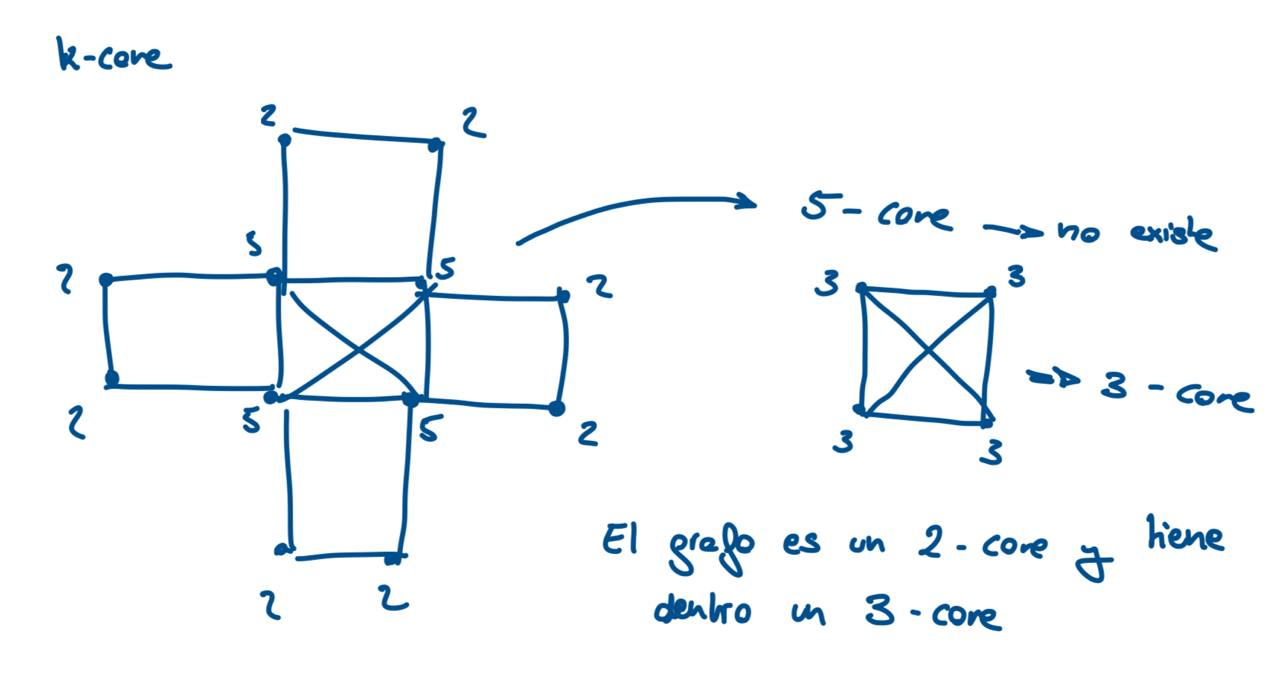
\includegraphics[width = 0.8\textwidth]{figs/kcore.jpg}
\end{figure}

\subsubsection{Operadores}
complement(G) devuelve el grafo complemento de G, y reverse(G[, copy]) el inverso del grafo dirigido G. compose(G, H) devuelve el grafo G compuesto con H, es decir, une los conjuntos de vértices y ramas de ambos grafos, los grafos no tienen por qué ser disjuntos. union(G, H[, rename, name]) devuelve la unión de G y H, ambos grafos deben ser disjuntos. intersection(G, H) devuelve un grafo que contiene solo
los nodos que están a la vez en G y H. difference(G, H)Devuelve un grafo con las ramas que están en G pero no en H.

\subsubsection{Caminos mínimos}
Para grafos ponderados:
\begin{itemize}
\item shortest\_path(G[, source, target, weight]) calcula el camino más corto entre dos nodos dados.
\item all\_shortest\_paths(G, source, target[, weight]) calcula todos los caminos mínimos en el grafo entre source y target.
\item shortest\_path\_length(G[, source, target, weight]) calcula la longitud del camino mínimo entre dos nodos dados.
\item average\_shortest\_path\_length(G[, weight]) calcula la el camino mínimo promedio del grafo(parámetro L).
\item has\_path(G, source, target) devuelve True si existe un camino entre source y target.
\item dijkstra\_path(G, source, target[, weight]) calcula el camino ponderado más corto entre source y target.
\item dijkstra\_path\_length(G, source, target[, weight]) calcula la longitud del camino ponderado más corto entre source y target.
\item dijkstra\_predecessor\_and\_distance(G, source) calcula el camino ponderado más corto y los predecesores desde source.
\item single\_source\_dijkstra(G, source[, target, …]) calcula el camino ponderado más corto y las distancias desde source.
\item single\_source\_dijkstra\_path(G, source[, …]) calcula el camino ponderado más corto desde source.
\item single\_source\_dijkstra\_path\_length(G, source) calcula las distancias desde source.
\end{itemize}

Para grafos no ponderados:
\begin{itemize}
\item single\_source\_shortest\_path(G, source[, cutoff]) calcula el camino más corto entre source y el resto de nodos del grafo.
\item single\_source\_shortest\_path\_length(G, source) calcula la longitud del camino más corto entre source y el resto de nodos alcanzables del grafo.
\item all\_pairs\_shortest\_path(G[, cutoff]) calcula el camino más corto entre todas las parejas de nodos del grafo.
\item all\_pairs\_shortest\_path\_length(G[, cutoff]) calcula la longitud del camino más corto entre todas las parejas de nodos del grafo.
\end{itemize}

\subsubsection{Algoritmos aproximados}
Muchos de los algoritmos vistos en las anteriores secciones son terriblemente lentos y otros incluso no se implementan por su enorme lentitud. Para solucionar este problema se recurre a algoritmos aproximados:
\begin{itemize}
\item max\_clique(G) encuentra el máximo cliqué 
\item average\_clustering(G[, trials]) estima el coeficiente de clustering C.
\item k\_components(G, min\_density=0.95) una k-componente es una componente que necesita eliminar al menos k nodos para desconectarse.
\item all\_pairs\_node\_connectivity(G, nbunch=None, cutoff=None) la conectividad entre dos nodos es el mínimo número de nodos que es necesario remover para desconectarlos.
\item astar\_path(G, source, target[, heuristic, …]) devuelve el camino más corto entre source y target según el algoritmo A*
\end{itemize}
